\documentclass{article}
\usepackage{amsmath}
\usepackage{placeins}
\usepackage{relsize,mathtools}
\usepackage{amsthm}
\usepackage{amsfonts}
\usepackage{ifthen}
\usepackage{mathdots}
\usepackage{amssymb}
\usepackage{cancel}
\usepackage{tikz}
\usetikzlibrary{positioning}
\usepackage[top=0.7in, bottom=1in, left=1in, right=1in]{geometry}
\renewcommand{\L}{\overline{L}}
\renewcommand\Pr[1]{\begingroup
    \renewcommand\mid{\;|\;}
    \text{P({\larger[2]$\scriptstyle#1$})}
    \endgroup}
\newtheorem{claim}{Claim}
\numberwithin{equation}{section}


\begin{document}
\title{Effects of overkill and regeneration on damage output rate in Oldschool Runescape}
\author{Nukelawe}
\date{\today}
\maketitle
\section{Introduction}\label{chap:introduction}
\section{Introduction}
Efficient combat training in Oldschool Runescape is a problem of maximizing the damage output rate of the player (often measured by DPS). To optimize the DPS it is important to be able to determine its value also theoretically. Overkill and hitpoint regeneration are two major factors that have significant effects on DPS, yet the quantitative understanding of them is limited.
While simulations provide quite good results, a more mathematical viewpoint can give further insight into the nature of these effects and result in some convenient approximations.

Overkill is an effect that occurs when the damage roll exceeds the remaining hitpoints of the enemy. It is important in combat training when the idle time between kills is short, and especially when the max hit is large relative to the enemy hitpoints.

The other mechanic that will be studied is health regeneration. Assuming no regeneration is a fair approximation when regeneration rate is much slower than the damage rate. But there are inevitably scenarios where this is not the case. Whereas overkill is most significant for high damage rates, regeneration affects mostly the slower fights. While there are many ways to regain health, we will be focusing on \textit{natural regeneration} only.


\section{Fight mechanics}\label{chap:fightMechanics}
A fight consists of two parties, the attacker and the enemy. We only consider the damage dealt by the attacker on the enemy and not vice versa. In our model the enemy is attacked periodically until its remaining hitpoints are 0. The attack rate is characterized by the \textit{attack period} $T_A$ which varies between weapons.
Once every attack period the enemy is hit and the damage dealt is calulated as follows.
\begin{enumerate}
	\item The game determines if the hit will succeed by some random process which depends on various parameters, such as defensive bonuses of the enemy, offensive bonuses of the attacker and appropriate combat-related stats. We ignore the details of this process and just say the probability of the hit being successful is $a$ calling it the \textit{accuracy}. If the accuracy check fails, the attack is considered a miss and 0 damage is dealt.
	\item If the accuracy check is successful damage roll $M$, a uniformly distributed random integer between 0 and $m$ is chosen, where $m$ is the \textit{maximum hit}. Again, we do not concern ourselves with the specifics of how the max hit is determined. Notice that it is possible for the hit to deal no damage even if the accuracy check succeeds because the damage roll $M$ could be 0.
    \item If $M > H$, where $H$ is the remaining hitpoints of the enemy, the damage is capped to $H$ and the final damage dealt is $\min(M,H)$. This is the overkill effect.
\end{enumerate}

Unlike the damage calculation process, regeneration is not fundamentally random. It happens by periodically incrementing the remaining hitpoints by one until they are full. The period $T_R$ of this healing cycle is called the \emph{regeneration period} and can vary between enemies giving rise to different regeneration rates. At the beginning of a fight the state of the healing cycle can be assumed to be unknown and thus treated as a random variable. This way only the timing of the first heal is random and the rest are perfectly periodic.


\section{No regeneration}\label{chap:noregen}
\subsection{Fight model}\label{chap:fightModel}
We define the \textit{state space} as the set of all possible values the remaining hitpoints of the enemy can have during a fight. For a fight against an enemy with $h$ maximum hitpoints the state space is $\{0,\ldots,h\}$. Each hit corresponds to a transition from one state to another in the state space. The probability of transitioning to state $i$ from state $j$ is called the \textit{transition probability} and is defined as
\begin{align}\label{eq:transitionProbabilities}
    p_{ij} = \Pr{H_k = i \mid H_{k-1} = j}.
\end{align}

Let $H_k$ be the number of hitpoints the enemy has remaining after $k$ hits. A fight can be labeled with a sequence of visited hitpoint states $(H_k)_{k=0}^{n}$. For the sequence to constitute a valid $n$-hit fight we must have $H_n=0$ (fight ends in death) and $h \geq H_k > 0$ for $k<n$ (death does not happen before the last hit). As an example consider a 4-hitpoint enemy that the attacker hits 3 times, first 1, then 0 and finally 3 damage killing the enemy. This fight would be described by the sequence $4,3,3,0$ and corresponds to the highlighted path in the state space diagram in Figure~\ref{fig:stateSpace}.
\begin{figure}[h]
    \centering
    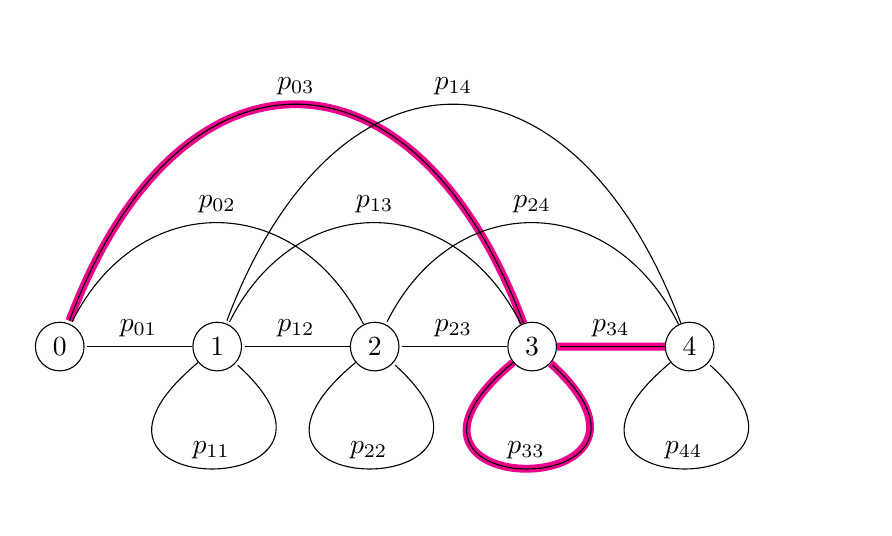
\begin{tikzpicture}[shorten >=1pt,node distance=1cm]
        \tikzstyle{state}=[shape=circle,draw,minimum size=1cm];
        \coordinate (n0);
        \xdef\scale{2}
        \xdef\maxhit{3}
        \foreach \s in {0,1,2,3,4} {
            \node[shape=circle,draw](n\s) at (\scale*\s,0){$\s$};
        }
		\path[draw, color=magenta, line width=1mm] (n4) ..
		controls({(0.75*4+0.25*3)*\scale},{2*(4-3-1)}) and ({(0.25*4+0.75*3)*\scale},{2*(4-3-1)})
		.. (n3) ..
        controls({(3-1.2)*\scale},-2) and ({(3+1.1)*\scale},-2)
		.. (n3) ..
		controls({(0.75*3+0.25*0)*\scale},{2*(3-0-1)}) and ({(0.25*3+0.75*0)*\scale},{2*(3-0-1)})
		.. (n0);
        \foreach \from in {1,2,3,4} {
            \foreach \to in {0,1,2,3,4} {
                \foreach \y [evaluate=\y as \yeval using \from-\to] in {1} {
                \foreach \m [evaluate=\m as \meval using int(\to+\maxhit+1)] in {1} {
                    \ifthenelse{\from>\to \AND \from<\meval \AND \to>0}{
                        \path[draw] (n\from) ..
                        controls({(0.75*\from+0.25*\to)*\scale},{2*(\from-\to-1)}) and ({(0.25*\from+0.75*\to)*\scale},{2*(\from-\to-1)})
                        .. node[above]{$p_{\to\from}$} (n\to);
                    }{}
                    \ifthenelse{\to=0 \AND \from<\meval}{
                        \path[draw] (n\from) ..
                        controls({(0.75*\from+0.25*\to)*\scale},{2*(\from-\to-1)}) and ({(0.25*\from+0.75*\to)*\scale},{2*(\from-\to-1)})
                        .. node[above]{$p_{\to\from}$} (n\to);
                    }{}
                    \ifthenelse{\from=\to}{
                        \path[draw] (n\from) ..
                        controls({(\to-1.2)*\scale},-2) and ({(\to+1.1)*\scale},-2) .. node[above]{$p_{\to\from}$} (n\to);
                    }{}
                }
                }
            }
        }
    \end{tikzpicture}\caption{State space diagram for $m=3$, $h=4$ and no regeneration. The probability of moving to state $i$ from state $j$ is given with the transition probability $p_{ij}$. Only edges for which $p_{ij} > 0$ are shown.}
	\label{fig:stateSpace}
\end{figure}

\subsection{Expected length of a fight}\label{chap:noregenRecurrences}
Let a fight's length $L_j$ be the number of hits to kill an enemy with $j$ hitpoints remaining. Its expected value $\E{L_j}$ is of fundamential importance to the derivation of many other interesting quantities. We will now derive a recurrence relation for it using the fight model described in Chapter~\ref{chap:fightModel}.

Let $\mathcal{S}_j^n$ be the set of all possible $n$-hit fights against an enemy with $j$ hitpoints remaining. The simplest possible case are the 1-hit fights $\mathcal{S}_j^1 = \{(j,0)\}$. The sets of all longer fights can be defined recursively by noticing that if the first hit lowers the hitpoints to $i$, the remaining sequence of states is equivalent to a fight of length $n-1$ against an enemy with $i$ hitpoints remaining. In other words
\begin{align}
	\mathcal{S}_j^n &=  \{j\} \times \bigcup_{i=1}^h \mathcal{S}_i^{n-1} \quad \mbox{for } n>1.\label{eq:fightRecursion}
\end{align}
For the set of all 2-hit fights this gives $\mathcal{S}_j^2 = \{(j,h,0), (j,h-1,0), \ldots, (j,2,0), (j,1,0)\}$. Notice that eq\ref{eq:fightRecursion} also allows transitions in which the enemy hitpoints increase. This will be useful when regeneration is considered in Chapter~\ref{chap:regen}.

Using the transition probabilities (eq\ref{eq:transitionProbabilities}) the probability that a particular $n$-hit fight $H \in \mathcal{S}_{j}^n$ occurs is
\begin{align}
    \Pr{H} &= \prod_{k=1}^{n} p_{H_{k} H_{k-1}}
\end{align}
The probability of a 1-hit fight is now
\begin{align}\label{eq:probabilityRecursion1hit}
    \Pr{L_j = 1} &= \sum_{\mathclap{H \in \mathcal{S}_j^1}}\Pr{H}
            = \Pr{(j,0}) = p_{0j}
\end{align}
For longer fights the probability is obtained by summing over all fights of length $n$ and invoking eq\ref{eq:fightRecursion}.
\begin{align}\label{eq:probabilityRecursion}
    \Pr{L_j = n} &= \sum_{\mathclap{H \in \mathcal{S}_j^n}}\Pr{H}
            = \sum_{i=1}^h p_{ij} \sum_{H \in \mathcal{S}\mathrlap{_i^{n-1}}}\Pr{H}
            = \sum_{i=1}^h p_{ij} \Pr{L_i = n-1}
\end{align}

The expected length of a fight can now be expressed as
\begin{align}
	\langle L_j \rangle &= \sum_{n=1}^{\infty}n\Pr{L_j=n}\nonumber\\
       &= \Pr{L_j=1} + \sum_{n=2}^{\infty}n\sum_{i=1}^h p_{ij} \Pr{L_i=n-1}\nonumber\\
       &= p_{0j} + \sum_{i=1}^h p_{ij} \sum_{n=2}^{\infty}n\Pr{L_i=n-1}.\label{eq:derivation2}
\end{align}
The inner sum can be worked out to be
\begin{align}
    \sum_{n=2}^{\infty}n\Pr{L_i=n-1}
       &= \sum_{n=1}^{\infty}(n+1)\Pr{L_i=n} \nonumber\\
	   &= \sum_{n=1}^{\infty}n\Pr{L_i=n} + \sum_{n=1}^{\infty}\Pr{L_i=n}\nonumber\\
	   &= \langle L_i \rangle + 1.
\end{align}
In the last equality we used the definition of expected value as well as the fact that an enemy will be guaranteed to die if hit infinitely many times. Inserting this back into eq\ref{eq:derivation2} gives
\begin{align}
    \langle L_j \rangle
        &= p_{0j} + \sum_{i=1}^h p_{ij}(\langle L_i \rangle+1)
        = \sum_{i=0}^h p_{ij} + \sum_{i=1}^h p_{ij}\langle L_i \rangle
\end{align}
Since the transition probabilities must add up to 1 when summed over the entire state space, we have $\sum_{i=0}^{h}p_{ij} = 1$ and the recurrence relation for the expected length of a fight becomes
\begin{align}
	\langle L_j \rangle
		= 1 + \sum_{i=1}^h p_{ij}\langle L_i \rangle.
	\label{eq:fightLengthRecursion}
\end{align}

To compute the length of a fight from the recurrence (eq\ref{eq:fightLengthRecursion}) we need to know the transition probabilities. From the fight mechanics as stated in Chapter~\ref{chap:fightMechanics} we can determine the probability distribution of the accuracy-corrected damage roll $X$. This is the amount of damage that would be dealt if the enemy had enough hitpoints to receive it (i.e.\ without considering overkill).
\begin{align}
	\Pr{X = k} =
	\begin{cases}
		1 - \frac{am}{m+1}, &\mbox{if } k = 0 \\
		\frac{a}{m+1},      &\mbox{if }1 \leq k \leq m\\
		0,      			&\mbox{if }k > m
	\end{cases}\label{eq:damageRollDistribution}
\end{align}
Here $a$ is the accuracy and $m$ the maximum hit as defined in Chapter~\ref{chap:fightMechanics}. In terms of eq\ref{eq:damageRollDistribution} the transition probabilities are given by
\begin{align}
    p_{ij}
         &= \begin{cases}
            \Pr{X=\,j-i} \quad &\mbox{if } i > 0 \\
            \Pr{X\geq\,j-i} \quad &\mbox{if } i = 0
        \end{cases}\label{eq:noregenProb}.
\end{align}

A nice feature of the transition probabilities for the regenerationless case is that the hitpoints can never increase because $p_{ij} = 0$ for $i > j$. In other words, it is impossible for the enemy hitpoints to climb up the state space. Thus, it makes no difference if the enemy being fought has full hitpoints or if some of them are already lost. In the absence of regeneration a fight against an enemy with $j$ hitpoints remaining is identical to a fight against an enemy whose maximum hitpoints \emph{are} $j$. Therefore, we can without loss of generality assume $j=h$ studying only fights that start at maximum hitpoints.

With these remarks, the transition probabilities can be inserted to eq\ref{eq:fightLengthRecursion} to obtain
\begin{align}
	\E{L_h}
		&= 1 + \sum_{i=1}^h \Pr{X=\,h-i}\E{L_i}\nonumber\\
		&= 1 + \Pr{X=\,0}\langle L_h \rangle + \sum_{i=1}^{h-1} \Pr{X=\,h-i}\langle L_i \rangle\nonumber\\
	\implies \frac{am}{m+1}\langle L_h \rangle
		&= 1 + \frac{a}{m+1}\sum_{i=h-m}^{h-1} \E{L_i}\nonumber\\
	\implies \langle L_h \rangle
		&= \frac{m+1}{am} + \frac{1}{m}\sum_{i=\max(1,h-m)}^h \E{L_i}\label{eq:recurrencetemp}
\end{align}
To simplify the summation limits in eq\ref{eq:recurrencetemp} we define $\langle L_i \rangle = 0$ for $i \leq 0$. Finally, by reversing the order of summation we get the recurrence relation
\begin{align}
	\boxed{\E{L_h}
		= \frac{m+1}{am} + \frac{1}{m}\sum_{i=1}^m \E{L_{h-i}}.
	}\label{eq:noregenRecursion}
\end{align}

\subsection{Explicit solution}\label{chap:noregenSolution}
\section{Solving the recurrences}\label{chap:recurrenceAnalysis}

In Chapter~\ref{chap:noregen} we obtained the length of a fight in terms of the recurrence relations
\begin{align}\label{eq:complexRecurrence1}
	\L_h = \begin{cases}
        \frac{m+1}{m}\L_{h-1} - \frac{1}{m}\L_{h-m-1} &\quad \mbox{if } h > m+1\\
        \frac{m+1}{m}\L_{h-1} &\quad \mbox{if } h \leq m+1
    \end{cases}
\end{align}
and the initial condition $L_1 = \frac{m+1}{ma}$. The case $h \leq m+1$ is simply the recurrence relation for a geometric sequence. Therefore,
\begin{align}
    \overline{L}_h &= \frac{1}{a} {\left( \frac{m+1}{m} \right)}^h \quad \mbox{if } h \leq m+1.\label{eq:geomProgression}
\end{align}

The recurrence relation for the case $h > m+1$ is not as easy to bring in a non-recursive form. It is a linear recurrence of order $m$, the initial $m$ elements of which are given by eq\ref{eq:geomProgression}. Inspired by the geometric progression, we define
\begin{align}
	r &= \frac{m+1}{m} \quad \mbox{and } \quad p = \frac{-1}{m+1}
\end{align}
and restate the recurrence relation and its initial condition a bit more neatly.
\begin{align}\label{eq:complexRecurrence2}
	\L_h = \begin{cases}
        r\left(\L_{h-1} - p\L_{h-m-1}\right) &\quad \mbox{if } h \leq m+1\\
        \frac{1}{a}r^h &\quad \mbox{if } h > m+1
    \end{cases}
\end{align}

This recurrence is perhaps most effectively approached with generating functions. The ordinary generating function of the number sequence $\L_h$ is a the function $g(z)$ whose power series expansion has $\L_h$ as coefficients.
\begin{align}
    g(z) = \sum_{h=1}^{\infty} \L_h z^h
\end{align}
Using the generating function formulation the recurrence (eq\ref{eq:complexRecurrence2}) translates into an algebraic equation for $g(z)$. Usually, for linear recurrences one would save some work by directly writing down the charasteristic polynomial $1 - rz - rpz^{m+1}$ and considering the initial values. For completeness, the full derivation will be given. It is straightforward but quite tedious, so feel free to skip ahead to the result (eq\ref{eq:ogf}).
\begin{align}
    g(z) &= \sum_{h=1}^{m+1} \L_h z^h + \sum_{h=m+2}^{\infty} \L_h z^h\nonumber\\
         &= \sum_{h=1}^{m+1} \L_h z^h + \sum_{h=m+2}^{\infty} r\left(\overline{L}_{h-1} + p\overline{L}_{h-m-1}\right)z^h\nonumber\\
         &= \sum_{h=1}^{m+1} \L_h z^h + rz\sum_{h-1=m+1}^{\infty}\overline{L}_{h-1}z^{h-1} + rpz^{m+1}\sum_{h-m-1=1}^{\infty}\overline{L}_{h-m-1}z^{h-m-1}\nonumber\\
         &= \sum_{h=1}^{m+1} \L_h z^h + rz\sum_{h=m+1}^{\infty}\overline{L}_{h}z^{h} + rpz^{m+1}\sum_{h=1}^{\infty}\overline{L}_{h}z^{h}\nonumber\\
         &= \sum_{h=1}^{m} \L_h z^h + \L_{m+1} z^{m+1} + rz\left(- \sum_{h=1}^{m}\overline{L}_{h}z^{h} + \sum_{h=1}^{\infty}\overline{L}_{h}z^{h}\right) + rpz^{m+1}g(z)\nonumber\\
         &= (1 - rz)\sum_{h=1}^{m} \L_h z^h + \L_{m+1} z^{m+1} + \left(rz + rpz^{m+1}\right)g(z)
\end{align}
Now, moving all terms containing $g(z)$ to the left and substituting the values for $\L_h$ from eq\ref{eq:geomProgression} gives
\begin{align}
    (1 - rz - rpz^{m+1})g(z) &= \frac{1}{a}\left({(rz)}^{m+1} + (1 - rz)\sum_{h=1}^{m} {(rz)}^h\right)\label{eq:ogfderiv1}
\end{align}
The partial sum on the right is the $m$ first terms of a geometric series which has the following closed form expression.
\begin{align*}
    \sum_{h=1}^{m} {(rz)}^h = rz\frac{1 - {(rz)}^m}{1-rz}
\end{align*}
Plugging it back to eq\ref{eq:ogfderiv1} to gives
\begin{align}
    (1 - rz - rpz^{m+1})g(z) &= \frac{1}{a}\left({(rz)}^{m+1} + rz\left(1 - {(rz)}^m\right)\right)\nonumber
                            = \frac{1}{a}rz\nonumber
                            = \L_1 z\nonumber\\
    \implies           g(z) &= \frac{\L_1 z}{1 - rz - rpz^{m+1}}\label{eq:ogf}.
\end{align}

To read off the explicit formula for $\L_h$ the generating function must be expanded back into a power series. This is possible by noticing that $g(z)$ is an infinite geometric sum with $rz(1 - pz^m)$ as its coefficient.
\begin{align}
    g(z) &= \frac{\L_1 z}{1 - rz\left(1 + pz^{m}\right)}\nonumber
    = \L_1 z\sum_{n=0}^\infty {(rz(1 + pz^m))}^n\nonumber
    = \frac{1}{a} \sum_{n=0}^\infty {(rz)}^{n+1}{(1 + pz^m)}^n
\end{align}
Then, we expand the $n$th order binomial term using the binomial theorem.
\begin{align}
    g(z) &= \frac{1}{a} \sum_{n=0}^\infty {(rz)}^{n+1}\sum_{i=0}^{n} {(pz^m)}^i {n \choose i}\nonumber\\
         &= \sum_{n=0}^\infty \frac{1}{a}\sum_{i=0}^{n} r^{n+1} p^i {n \choose i}z^{mi+n+1}\label{eq:ogf2}.
\end{align}
$\L_h$ is now the coefficient of the term $z^h$. Looking at the exponent of $z$ in eq\ref{eq:ogf2} we see that for the coefficient of interest the indices $i$ and $n$ must satisfy $h=mi+n+1$. For each $i$ there is exactly one valid $n$, namely $n = h-mi-1$.
Therefore, the coefficient of the $h$th order term in the series expansion of $g(z)$ is
\begin{align}
    \L_h &= \frac{1}{a}\sum_{i \in \mathcal{I}} r^{h-mi} p^i {h-mi-1 \choose i} \nonumber
\end{align}
where $\mathcal{I}$ is the set of indices $i$ such that
\begin{align*}
    0 \leq i \leq n = h-mi-1
    \iff (m+1)i \leq h-1
    \iff i \leq \frac{h-1}{m+1}.
\end{align*}
Since $i$ must also be an integer the index set becomes $\mathcal{I} = \left\{0,1,\ldots,\left\lfloor{\frac{h-1}{m+1}}\right\rfloor\right\}$. Expressing the constants $r$ and $p$ explicitly, the solution to the recursion problem (eq\ref{eq:complexRecurrence2}) can be written as
\begin{align}
    \L_h &= \frac{1}{a}\sum_{i=0}^{\left\lfloor{\frac{h-1}{m+1}}\right\rfloor} {\left(\frac{m+1}{m}\right)}^{h-mi} {\left(\frac{-1}{m+1}\right)}^i {h-mi-1 \choose i}.\label{eq:explicitL}
\end{align}
Naturally this can also be proven to satisfy the recursion using induction (see Appendix~\ref{sect:genLProof}). With this result the damage dealt per hit is simply $h/\L_h$ and the damage per second can be obtained from it by dividing with the attack interval $T_A$.

Eq\ref{eq:explicitL} can be annoying to work with, especially for large $h$, so an approximation for the case $h \gg m$ is needed. Intuitively the length of a fight should have linear dependency on hitpoints as $h \rightarrow \infty$. This is because on average one can expect each hit to do $am/2$ damage and therefore it should take approximately $2h/am$ hits to kill an enemy with $h$ hitpoints. Due to overkill however, the last hit will do slightly less than $am/2$ damage on average introducing a constant correction term to this linear approximation.
The average length of a fight with no regeneration has the following asymptotic behaviour (derivation not shown here).
\begin{align}\label{eq:asymptoticAppr}
\L_h \sim \frac{2}{ma}\left(h + \frac{m-1}{3}\right)
\end{align}
The correctness of both the results was validated by comparing them to a computer simulation. The comparison is illustrated in figure~2.
\begin{figure}[t]\label{fig:apprComparison}
    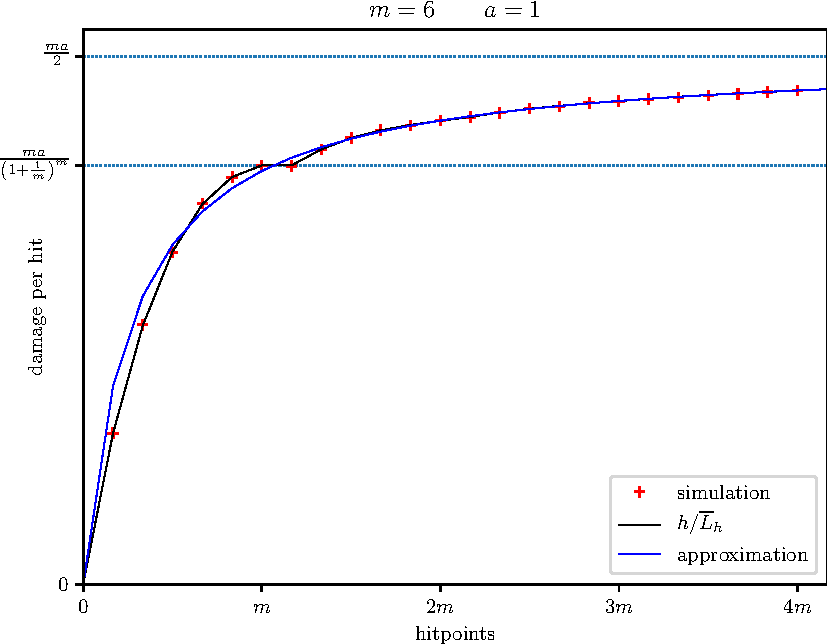
\includegraphics[scale=1.1]{dph-appr-m6.pdf}
    \caption{Comparison of damage per hit (DPH) calculated using the explicit formula (eq\ref{eq:explicitL}), asymptotic approximation (eq\ref{eq:asymptoticAppr}) and a simulation. The simulation was written using the damage calculation mechanics described in Chapter~\ref{chap:fightDef}. For each datapoint $10^{5}$ fights were simulated and their average lengths calculated.}
\end{figure}

\subsection{Asymptotic approximation}\label{chap:noregenAsymptotics}
\subsection{Asymptotic approximation}
Eq\ref{eq:explicitL} can be annoying to work with, especially for large $h$, so an approximation for the case $h \gg m$ is needed. Intuitively the length of a fight should have linear dependency on hitpoints as $h \rightarrow \infty$. This is because on average one can expect each hit to do $am/2$ damage and therefore it should take approximately $2h/am$ hits to kill an enemy with $h$ hitpoints. Due to overkill however, the last hit will do slightly less than $am/2$ damage on average introducing a constant correction term to this linear approximation.
%Since eq\ref{eq:explicitL} is tricky to approximate we take a completely different approach and try to look at the damage per hit directly instead of trying to approximate $\L_h$. Recall the definition of a fight as a sequence of damage rolls $\{X_i\}$. The total damage dealt by these hits is $\sum X_i = h$, but because of overkill the last hit contributes less to this sum than the others. To find the magnitude of this discrepancy, let us ignore all the hits that deal no damage to obtain a sequence of non-zero hits, $\{Z_i\}$. This is a subsequence of $\{X_i\}$ and its elements have the following probabilities, where $H_i$ is the remaining hitpoints after $i$ \textit{non-zero} hits.
%\begin{align}
%    \Pr{Z_i = k \mid H_{i-1} = l} = \begin{cases}
%        \frac{1}{m}, &\quad\mbox{if } k < l\\
%        \frac{m-k+1}{m}, &\quad\mbox{if } k = l\\
%        0, &\quad\mbox{if } k > l \quad \mbox{or } k \notin [1,m]
%    \end{cases}
%\end{align}
%The probability distribution of $H_i$ is given recursively for $i \geq 1$ and $k > 0$.
%\begin{align}
%    \Pr{H_i = k} &= \sum_{j\geq 1} \Pr{Z_i = j \mid H_{i-1} = k+j}\Pr{H_{i-1} = k+j} = \frac{1}{m}\sum_{j=1}^m \Pr{H_{i-1} = k+j}
%\end{align}
%The case $k=0$ is interesting since $\Pr{H_i = 0} = \Pr{L_h = i}$. This is given by
%\begin{align}
%    \Pr{H_i = 0} &= \sum_{j\geq 1} \Pr{Z_i = j \mid H_{i-1} = j}\Pr{H_{i-1} = j} = \sum_{j=1}^m \frac{m-j+1}{m}\Pr{H_{i-1} = k+j}
%\end{align}
%Since every fight starts at $h$ hitpoints the inital condition is $\Pr{H_0=k} = \delta_{k,h}$, where $\delta_{k,h}$ is the Kronecker delta.
%
%We say that the state $k$ is visited if there exists $i \in \mathbb{N}_0$ such that $H_i = k$. This is the same as saying that at some point during the fight the enemy had $k$ hitpoints remaining. Let $\Pr{V_k}$ be the probability of visiting state $k$. For the initial and final states we have $\Pr{V_h} = \Pr{V_0} = 1$ and between them the visiting probability can be specified recursively.
%\begin{align}
%    \Pr{V_k} &= \sum_{i \geq 0} \Pr{H_i = k} = \frac{1}{m}\sum_{j=1}^m \sum_{i \geq 0} \Pr{H_{i-1} = k+j}\nonumber\\
%            &= \frac{1}{m}\sum_{j=1}^m \left(\Pr{H_0 = k+j} + \sum_{i \geq 1} \Pr{H_{i-1} = k+j}\right)\nonumber\\
%            &= \frac{1}{m}\sum_{j=1}^m \left(\delta_{k+j,h} + \sum_{i \geq 0} \Pr{H_{i} = k+j}\right)
%            = \frac{1}{m}\sum_{j=1}^m \left(\delta_{k+j,h} + \Pr{V_{k+j}}\right)\label{eq:vkgen}
%\end{align}
%
%The plan is now to show the existence and find the value of the limit of $\Pr{V_k}$ as $h \rightarrow \infty$ for any fixed $k$. First, we claim that $\Pr{V_k}$ increases as $k$ decreases. Clearly this is not true for the initial state $k=h$ because it is always visited, but for all the lower states we should have
%\begin{claim}\label{claim:vkhinc}
%    $\Pr{V_{k-1}} > \Pr{V_k}$ \quad for $0 < k < h$.
%\end{claim}
%\begin{proof}
%Eq\ref{eq:vkgen} gives
%\begin{align}
%    \Pr{V_{k-1}} &= \frac{1}{m}\sum_{j=1}^m \left(\delta_{(k-1)+j,h} + \Pr{V_{(k-1}+j})\right)\label{eq:proof321}.
%\end{align}
%Consider the case $h - m < k < h$. If $k-1+j > h$ then $\Pr{V_{k-1+j}} = 0$ since the hitpoints of the enemy can never exceed $h$. Therefore, the terms in eq\ref{eq:proof321} for which $j>h-(k-1)$ can be dropped.
%The sum over the Kronecker deltas can be evaluated by noticing that for any $k$ in the range under consideration there is exactly one $j$ for which $k-1+j = h$. With these remarks eq\ref{eq:proof321} can be written as
%\begin{align}
%    \Pr{V_{k-1}} &= \frac{1}{m}\left(1 + \sum_{j=1}^{h-(k-1)}\Pr{V_{(k-1}+j})\right)
%    = \frac{1}{m}\left(1 + \Pr{V_{k}} + \sum_{j=2}^{h-k+1}\Pr{V_{k-1+j}}\right)\nonumber\\
%              &= \frac{1}{m}\left(1 + \Pr{V_{k}} + \sum_{j=1}^{h-k}\Pr{V_{k+j}}\right)\nonumber
%              = \frac{1}{m}\Pr{V_{k}} + \frac{1}{m}\left(1 + \sum_{j=0}^{h-k}\Pr{V_{k+j}}\right)\\
%              &= \frac{1}{m}\Pr{V_{k}} + \Pr{V_{k}} \quad > \quad \Pr{V_{k}}.\label{eq:proof323}
%\end{align}
%This proves the statement for all $k$ in the range $h-m<k<h$ implying $\Pr{V_{h-m}} > \cdots > \Pr{V_{h-1}}$.
%
%Assume that $\Pr{V_{k}} >\cdots> \Pr{V_{k+m-1}}$ is true for some $k$ in the range $0 < k \leq h-m$. In this range the Kronecker delta terms in eq\ref{eq:proof321} vanish and $\Pr{V_{k}}$ is given as the average of the last $m$ terms.
%\begin{align}
%    \Pr{V_{k-1}} &= \frac{1}{m}\sum_{j=1}^m \Pr{V_{(k-1}+j})
%               = \frac{1}{m}\sum_{j=0}^m \Pr{V_{k+j}}
%               > \frac{1}{m}\sum_{j=0}^{m-1} \Pr{V_{k}} = \Pr{V_{k}}
%\end{align}
%We already proved the assumption $\Pr{V_{k}} >\cdots> \Pr{V_{k+m-1}}$ is true for $k=h-m$. By induction the chain of inequalities can therefore be extended to $\Pr{V_{1}} > \cdots > \Pr{V_{h-1}}$, which proves the claim.
%\end{proof}
%Saying that $k$ is decreasing is equivalent to saying that $h$ is increasing for some fixed $k$. Being a probability $\Pr{V_k}$ is also bounded by 1. Therefore the limit $\Pr{V} = \lim_{h \rightarrow \infty}\Pr{V_{k}}$ exists. To find the value of this limit we look at the event $V'_k$, that state $k$ is never visited (i.e skipped). In practice skipping state $k$ means there must be two successive states $H_i$ and $H_{i-1}$ of the fight such that $H_{i} < k < H_{i-1}$. The probability that state $k$ is skipped by jumping over it from state $k+j$ is
%\begin{align}
%    \Pr{V_{k+j}}\Pr{Z_i > j | H_{i-1} = k+j} = \Pr{V_{k+j}}\sum_{n=j+1}^{m}\frac{1}{m} = \Pr{V_{k+j}}\frac{m-j}{m}.
%\end{align}
%This is true regardless of \textit{when} the hitpoint state was visited (i.e for which $H_i$). Since state $k$ can be skipped by jumping over it from any of the states $\{k+1,\ldots,k+m-1\}$ we can write the probability of never visiting $k$ as
%\begin{align}
%    \Pr{V'_k} = 1-\Pr{V_{k}} = \sum_{j=1}^{m-1}\Pr{V_{k+j}}\frac{m-j}{m}.
%\end{align}
%If $\Pr{V}$ is the limit of $\Pr{V_k}$ as $h \rightarrow \infty$ then
%\begin{align}
%    1-\Pr{V} &= \Pr{V}\sum_{j=1}^{m-1}\frac{m-j}{m}
%           = \Pr{V}\sum_{j=1}^{m-1}\left(1 - \frac{j}{m}\right)
%           = \Pr{V}\left((m-1) - \frac{1}{m}\sum_{j=1}^{m-1}j\right)\nonumber\\
%           &= \Pr{V}\left((m-1) - \frac{1}{m}\frac{m(m-1)}{2}\right)
%           = \Pr{V}\frac{m-1}{2}\nonumber\\
%    \implies 1 &= \Pr{V}\left(\frac{m}{2} - \frac{1}{2} + 1\right) = \Pr{V}\frac{m+1}{2}\nonumber\\
%    \implies \Pr{V} &= \frac{2}{m+1}\label{eq:visitproblimit}
%\end{align}
%
%If the number of non-zero hits is $N$, then $Z_N = X_{L_h}$ because the last hit has to do at least $1$ damage by definition. Its expected value can be calculated from the visiting probabilites.
%\begin{align}
%    \overline{Z}_N &= \sum_{n \geq 1} n \Pr{Z_N = n}
%    = \sum_{n \geq 1} n \Pr{V_n} \Pr{Z_N = n \mid H_{N-1} = n}\nonumber\\
%                    &= \sum_{n=1}^{m} n \Pr{V_n} \frac{m-n+1}{m}
%                    = \frac{1}{m}\sum_{n=1}^{m}\Pr{V_n}\left((m+1)n - n^2\right) \nonumber
%\end{align}
%In the limit that $h \rightarrow \infty$ the visit probabilites will be given by eq\ref{eq:visitproblimit} and the expectation has the following limit.
%\begin{align}
%    \lim_{h \rightarrow \infty}\overline{Z}_N
%              &= \frac{1}{m}\sum_{n=1}^{m}\frac{2}{m+1} \left((m+1)n - n^2\right)
%              = \frac{2}{m(m+1)}\left((m+1)\sum_{n=1}^{m} n - \sum_{n=1}^{m} n^2\right)\nonumber\\
%              &= \frac{2}{m(m+1)}\left(\frac{m{(m+1)}^2}{2} - \frac{m(m+1)(2m+1)}{6}\right)\nonumber\\
%              &= \frac{m+1}{2} - \frac{2m+1}{6}
%              = \frac{3m+3 - 2m-1}{6}
%              = \frac{m+2}{6}\label{eq:lastHitDamage}
%\end{align}
%For all the hits except the last one the expected damage dealt is a constant. Namely
%\begin{align}
%    \overline{X}_i
%        &= \sum_{n \geq 1} n \Pr{X = n}
%        = \sum_{n = 1}^{m} n \frac{a}{m+1}
%        = \frac{a}{m+1}\frac{m(m+1)}{2}
%        = \frac{am}{2}\label{eq:otherHitDamage}
%\end{align}
%Comparing eq\ref{eq:lastHitDamage} and eq\ref{eq:otherHitDamage} tells us how overkill lowers the damage dealt per hit. In particular, notice that the last hit does not depend on accuracy because it has to kill the enemy. If overkill did not happen and the damage rolled by the last hit always exactly brought the enemy hitpoints to $0$ the damage dealt by the last hit would have the expected value $\frac{m}{2}$. Therefore, the extra damage that would have been dealt is $\frac{m}{2}-\frac{m+2}{6}=\frac{m-1}{3}$.
%If the expected damage dealt by all the hits, including the last one, was the one specified by eq\ref{eq:otherHitDamage}, then the hitpoints of the enemy would have to be corrected to $h+\frac{m-1}{3}$. This gives the asymptotic approximation for the average length of a fight.
The average length of a fight with no regeneration has the following asymptotic behaviour (derivation not shown here).
\begin{align}\label{eq:asymptoticAppr}
\langle L_h \rangle \sim \frac{2}{ma}\left(h + \frac{m-1}{3}\right)
\end{align}
The correctness of both the results was validated by comparing them to a computer simulation. The comparison is illustrated in figure~2.
\begin{figure}[t]\label{fig:apprComparison}
    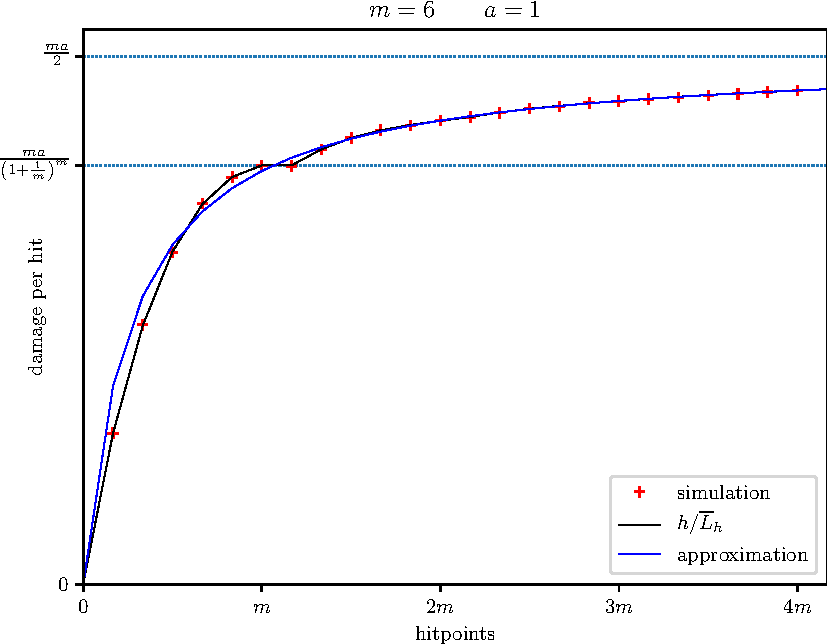
\includegraphics[scale=1.1]{dph-appr-m6.pdf}
    \caption{Comparison of damage per hit (DPH) calculated using the explicit formula (eq\ref{eq:explicitL}), asymptotic approximation (eq\ref{eq:asymptoticAppr}) and a simulation. The simulation was written using the damage calculation mechanics described in Chapter~\ref{chap:fightDef}. For each datapoint $10^{5}$ fights were simulated and their average lengths calculated.}
\end{figure}

%The approximation is clearly correct and converges quite quickly as can be seen from Figure~\ref{fig:apprComparison}. But the lack of rigour in the last few steps of deriving it calls for either a proof of its validity or a different derivation method. If eq\ref{eq:asymptoticAppr} really is an asymptotic approximation of $\L_h$ it should satisfy
%\begin{align}
%    \L_h - \frac{2}{ma}\left(h + \frac{m-1}{3}\right) \xrightarrow[h \rightarrow \infty]{} 0.
%\end{align}
%Unfortunately this could not be proven. One approach to it is using the explicit expression for $\L_h$ given by eq\ref{eq:explicitL}. However, this turns out to be quite tricky due to the binomial coefficients in the sum. It might be necessary to use generating functions or work directly with the defining recurrence relations (eq\ref{eq:complexRecurrence2}). The problem of finding the asymptotic behaviour of the recurrence is a purely mathematical one. Making heavy use of the properties of the underlying problem the recurrence is a solution for should not be necessary.
%\begin{figure}[t]\label{fig:apprComparison}
%    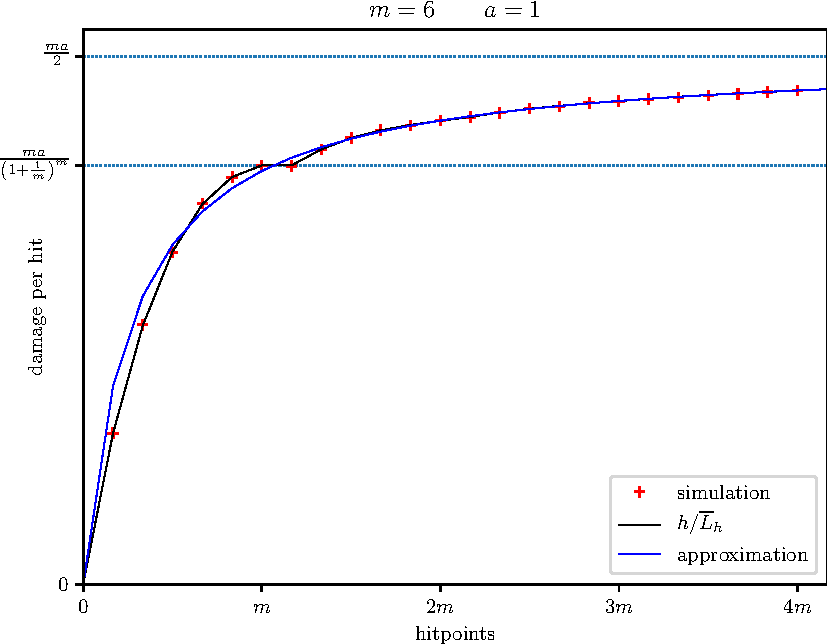
\includegraphics[scale=1.1]{dph-appr-m6.pdf}
%    \caption{Comparison of damage per hit (DPH) calculated using the explicit formula (eq\ref{eq:explicitL}), asymptotic approximation (eq\ref{eq:asymptoticAppr}) and a simulation. The simulation was written using the damage calculation mechanics described in Chapter~\ref{chap:fightDef}. For each datapoint $10^{5}$ fights were simulated and their average lengths calculated.}
%\end{figure}


\pagebreak
\section{Regeneration}\label{chap:regen}
\section{Regeneration}\label{chap:regen}
When regeneration is considered, the random walk that was used to describe a fight in Chapter~\ref{chap:fightDef} gets new edges. Now it will be possible to walk backwards as well as forwards in the state space. Unfortunately, the regeneration period $T_R$ and the attack interval $T_A$ are generally not equal. The attack and healing cycles will also go in and out of synchronization if the two periods are not integer multiples of one another. This makes the transition probabilities of the random walk no longer depend on just the current state and the Markov property is lost. This means we cannot use the methodology developed in Chapter~\ref{chap:fightDef}. However, the regeneration model described in Chapter~\ref{chap:fightMechanics} could be tweaked a bit to reattain the Markov property. The tweaked model can then be validated against a simulation that uses the more accurate regeneration mechanics.

Consider the time interval $\Delta t_k = [t_k, t_{k+1}-1]$, where $t_k$ is the game tick on which the $k$th hit occurs. By choosing $t_0 = 0$, the time interval can be written as
\begin{align}
	\Delta t_k = [kT_A, (k+1)T_A - 1].
\end{align}
The random walk approach described in Chapter~\ref{chap:fightDef} can be applied to fights with regeneration by letting a step correspond to the overall state change in the time interval $\Delta t_k$. If we assume that $T_R \geq T_A$ the number of regeneration attempts during $\Delta t_k$ is either 1 or 0 depending on the phase of the regeneration cycle. If the time at which the first regeneration occurs is $\tau$ then a regeneration attempt occurs during $\Delta t_k$ if and only if there exists $n \in \mathbb{N}_0$ such that
\begin{align}
	kT_A \leq \tau& + nT_R \leq (k+1)T_A - 1\\
	\iff kT_A - nT_R \leq \tau& \leq kT_A - nT_R + T_A - 1
\end{align}
the number $n$ can be further constrained by using the fact that $0 < \tau \leq T_R$.
\begin{align}
	kT_A - nT_R &\leq \tau \leq T_R &\mbox{and}& &0 &< \tau \leq kT_A - nT_R + T_A - 1\\
	n &\geq \frac{kT_A}{T_R} - 1 && &n &< \frac{kT_A}{T_R} + \frac{T_A - 1}{T_R}
\end{align}
\begin{align}
	\frac{kT_A}{T_R} - 1 \leq n < \frac{kT_A}{T_R} + 1 - \frac{1}{T_R}
\end{align}

While treating the regeneration attempt probability between hits as random variables is true
The assumption $T_A \leq T_B$ should hold for nearly all cases in practice as the the typical regeneration period is 60 seconds and even the slowest weapons have attack periods of just 4.2 seconds. For some rarer cases such as flinching an enemy with unusually high regeneration rate where this could become a problem one could simply allow the regeneration of more than 1 hitpoint per attack interval.



The regeneration attempt fails if the enemy is either already dead or fully regenerated.

Instead of regenerating deterministically at realistic time intervals we could assume that the healing happens right after each hit with such a probability that the correct regeneration rate is achieved.

\begin{align}\label{eq:regenProbability}
    \rho = \frac{T_A}{T_R}.
\end{align}

When accounting for regeneration, there are two ways of lowering the hitpoints by $k$: hit $k$ and heal 0 or hit $k+1$ and heal 1. Since regeneration has no effect on 1-hit fights we take the result $\L_1 = \frac{m+1}{am}$ from Chapter~\ref{chap:noregen} and assume without loss of generality that $h>1$. In terms of the regeneration probability $\rho$ and the damage roll $X$ the transition probabilities are
\begin{align}
    p_{ij}
         &= \begin{cases}
			 \Pr{X = j-i} + \rho \Pr{X = j-i+1} \quad &\mbox{if } i = h \\
            (1-\rho)\Pr{X = j-i} + \rho \Pr{X = j-i+1} \quad &\mbox{if } 1 < i < h \\
            (1-\rho)\Pr{X = j-i} \quad &\mbox{if } i = 1 \\
            \Pr{X \geq j-i} \quad &\mbox{if } i = 0
        \end{cases}\label{eq:damageDistributionRegen}.
\end{align}
Notice that transitioning to state 0 does not depend on regeneration because dead enemies cannot regenerate. For the same reason it is impossible to land in state 1 by first reaching 0 hitpoints and then healing. Transition probability for going to state $h$ on the other hand, is different because it is not possible to heal past maximum hitpoints.

With regeneration taken into account it now makes a difference whether the enemy is at full hitpoints or not. For simplicity we will only be considering fights that start at full hitpoints and assume $j=h$. The transition probabilities can now be inserted to eq\ref{eq:fightLengthRecursion} and after a very tedious calculation (see Appendix~\ref{sect:regenRecurrenceDerivation}) one obtains the following recurrence.
\begin{align}\label{eq:regenLengthRecurrence}
    \L_h &= \begin{cases}
        \frac{m-\rho+1}{m-\rho}\L_{h-1} \quad &\mbox{if } h \leq m+1\\
        \frac{m-\rho+1}{m-\rho}\L_{h-1} - \frac{\rho}{m-\rho}\L_{h-m} - \frac{1-\rho}{m-\rho}\L_{h-m-1} \quad &\mbox{if } h > m+1
    \end{cases}
\end{align}
As expected, this reduces to the regenerationless case (eq\ref{eq:complexRecurrence1}) when $\rho=0$.

Unfortunately, knowing the length of a fight is not very useful for calculating the damage dealt per hit. Total damage dealt is no longer equal to the enemy hitpoints as there might have been regenerations. Furthermore, even if the number of healed hitpoints was known it would now be a random variable, so dividing its expected value by the expected length would no longer give the correct result. Nevertheless, eq\ref{eq:regenLengthRecurrence} still serves as a way of checking the validity of the tweaked regeneration model that was used to preserve the Markov property.

In this case it is better to try express damage per hit directly. Notice that as long as the enemy has more than $m$ hitpoints remaining the expected damage dealt by each hit is $\frac{ma}{2}$. The probability distribution of damage dealt by a hit only depends on how much below $m$ the current hitpoint state is.
Assuming there is no idle time between fights the random walk presented in Chapter~\ref{chap:fightDef} can be made cyclic by letting $h$ and $0$ represent the same state. This makes sense as long as the enemy is always immediately replaced by a new one once it dies. Finding the steady state of this cyclic random walk allows us to determine the proportion of hits that start from somewhere. Finding the steady state of this cyclic random walk allows us to determine the proportion of hits that start from somewhere.

\subsection{Regenerating random walker}\label{chap:regen-walker}
When regeneration is considered, the random walk that was used to describe a fight in Chapter~\ref{chap:fightModel} gets new edges. Now it will be possible to walk backwards as well as forwards in the state space. Unfortunately, since regeneration attempts happen with a fixed period $T_R$, the transition probabilities will vary with time. Furthermore, when the regeneration attempts do occur they might not coincide with the damaging events.

To incorporate the two events in the same random walker formalism, consider the time interval $\Delta t_k = [t_k, t_{k+1}-1]$, where $t_k$ is the (game)tick on which the $k$th hit occurs. A single transition of the random walker is now determined by the overall state change that takes place during time interval $\Delta t_k$. Since we have assumed $T_R \geq T_A$ the number of regeneration attempts during $\Delta t_k$ is at most 1.
The assumption $T_A \leq T_B$ should hold for nearly all cases in practice as the the typical regeneration period is 60 seconds and even the slowest weapons have attack periods of just 4.2 seconds. For some rarer cases such as flinching an enemy with unusually high regeneration rate where this could become a problem one could simply allow the regeneration of more than 1 hitpoint per attack interval.

The only source of randomness in the regeneration model is the tick $\tau$ on which the first regeneration attempt occurs. We treat it as a random variable distributed uniformly in the interval $[1, T_R]$. Alternatively $\tau$ can be thought of as the time until the next regeneration attempt at the beginning of a fight. Now the expected length of a fight is
\begin{align}
	\langle L_j \rangle
		&= \sum_{n=1}^{\infty}n\Pr{L_j=\,n}\nonumber\\
		&= \sum_{n=1}^{\infty}n\sum_{\tau=1}^{T_R}\Pr{\tau}\Pr{L_j=\,n \mid \tau}\nonumber\\
		&= \frac{1}{T_R}\sum_{\tau=1}^{T_R}\sum_{n=1}^{\infty}n\Pr{L_j=\,n \mid \tau}\nonumber\\
		&= \frac{1}{T_R}\sum_{\tau=1}^{T_R} \langle L_j^\tau \rangle
\end{align}
where $L_j^\tau$ is the length of a fight at the beginning of which the next regeneration attempt is $\tau$ ticks away. While not shown here, by almost identical reasoning to that in Chapter~\ref{chap:fightDef} one can derive the recurrence relation
\begin{align}\label{eq:regenrecurrence}
	\langle L_j^\tau \rangle
		&= 1 + \sum_{i=1}^{h} p_{ij}^\tau \langle L_i^{\tau - T_A} \rangle.
\end{align}
The only critical difference besides the transition probabilities is the recursion argument. Now in addition to modifying the remaining hitpoints, hitting the enemy also shifts $\tau$ backwards by $T_A$ ticks since this is the amount of time that passes between hits. The time-dependent transition probabilities are given by
\begin{align}
    p_{ij}^\tau
        &= \begin{cases}
			p_{ij} \quad &\mbox{if } \tau > T_A \pmod {T_R} \\
			p_{i,\min(j+1,h)} \quad &\mbox{if } \tau \leq T_A \pmod {T_R}
		\end{cases}\label{eq:damageDistribution}.
\end{align}
where $p_{ij}$ is the transition probability of the non-regenerating case (eq\ref{eq:noregenProb}). The minimum is taken to prevent hitpoints from exceeding $h$ and modular arithmetic used to handle the periodicity of the regeneration cycle.

Because of the backwards transition that regeneration has made possible, all states are now dependent on one another. Therefore, a recursive solution similar to that in Chapter~\ref{chap:noregen} is no longer possible and eq\ref{eq:regenrecurrence} should instead be treated as a linear system of $h$ equations. Furthermore, the time shift in the $\tau$-dependency splits them further making the system actually $hT_R/\gcd(T_R, T_A)$-dimensional.
For example in case of fighting ankous with a scimitar ($h=60$, $T_R=100$, $T_A=4$) we would have to solve a system of 1500 equations.

\subsection{Random healing cycle approximation}
Instead of regenerating deterministically at realistic time intervals we could assume that the healing happens right after each hit with such a probability that the correct regeneration rate is achieved. This reduces the complexity of equation~\ref{eq:regenrecurrence} significantly as it removes the $\tau$-dependence entirely. We define the \emph{regeneration rate} as
\begin{align}\label{eq:regenProbability}
    \rho = \frac{T_A}{T_R}
\end{align}
and interpret it as the probability that a regeneration event occurs during an attack cycle.

In this model, there are two ways of lowering the hitpoints by $k$: hit $k$ and heal 0 or hit $k+1$ and heal 1. In terms of the regeneration probability $\rho$ and the damage roll $X$ the transition probabilities are
\begin{align}
    p_{ij}
         &= \begin{cases}
			 \Pr{X = j-i} + \rho \Pr{X = j-i+1} \quad &\mbox{if } i = h \\
            (1-\rho)\Pr{X = j-i} + \rho \Pr{X = j-i+1} \quad &\mbox{if } 1 < i < h \\
            (1-\rho)\Pr{X = j-i} \quad &\mbox{if } i = 1 \\
            \Pr{X \geq j-i} \quad &\mbox{if } i = 0
        \end{cases}\label{eq:damageDistributionRegen}.
\end{align}
Notice that transitioning to state 0 does not depend on regeneration because dead enemies cannot regenerate. For the same reason it is impossible to land in state 1 by first reaching 0 hitpoints and then healing. Transition probability for going to state $h$ on the other hand, is different because it is not possible to heal past maximum hitpoints.

Naturally it is still possible for the remaining hitpoints to climb up the state space making a recursive solution impossible. However, because of the eliminated dependence on the pahse of the regeneration cycle the walker is now fully described by equation~\ref{eq:fightLengthRecursion} just like in the regenerationless case. This reduces the size of the linear system down to $h$ equations, which is a much more manageable number for practical calculations.

\subsection{Effective hitpoints approach}
Consider a fight of length $L$. Since the fight lasts $T_A L$ ticks the number of hitpoints regenerated can be estimated by $\frac{T_A}{T_R} L$. Assuming that the enemy has $h$ maximum hitpoints, the total damage dealt during the fight is $y \equiv h + \frac{T_A}{T_R} L$. This quantity is called the \textit{effective hitpoints} because the fight is nearly equivalent to one against a non-regenerating enemy with $y$ hitpoints. If regeneration rate is small compared to the damage rate the expected length of a fight should be approximately $\langle L_y \rangle$. This gives us the equation
\begin{align}\label{eq:effHp}
	y = h + \rho\langle L_y \rangle
\end{align}
where we have defined the \textit{regeneration rate} $\rho \equiv \frac{T_A}{T_R}$.

To solve $y$ from this equation we use the asymptotic approximation (eq\ref{eq:asymptoticAppr}).
\begin{align}
	y &= h + \frac{2\rho}{ma} \left(y + \frac{m-1}{3}\right)\nonumber\\
	\implies \left(1 - \frac{2\rho}{ma}\right) y &= h + \frac{2\rho}{ma} \frac{m-1}{3}\nonumber\\
	\implies y
		&= \frac{1}{ma - 2\rho}\left(mah + 2\rho \frac{m-1}{3}\right)\nonumber\\
		&= h + \rho\left(\frac{h + \frac{m-1}{3}}{\frac{ma}{2} - \rho}\right)
\end{align}
Writing the effective hitpoints in this form reveals some nice properties. Comparing the result to eq\ref{eq:effHp} allows reading off the expected length of a fight as
\begin{align}
	\langle L_y \rangle = \frac{h + \frac{m-1}{3}}{\frac{ma}{2} - \rho}
\end{align}
and in turn the damage per hit as
\begin{align}
	\frac{y}{\langle L_y \rangle}
		&= \frac{\frac{ma}{2} - \rho}{1 + \frac{m-1}{3h}} + \rho
\end{align}
If the regeneration rate $\rho$ is larger than the damage rate $\frac{ma}{2}$ the equation breaks down as the term $\frac{ma}{2} - \rho$ becomes negative. This seems to suggest that in this case the fight would go on forever. Of course this is just a limitation of the model since in reality the fight would eventually terminate as long as $T_R > T_A$ and $m > 0$, which is a very resonable assumption.


\section{Kill and damage rates}
Consider a sequence of $n$ fights and assume that throughout all of them the fight parameters $a$, $m$ and $h$ stay unchanged. If we denote the length of the $i$th fight in this sequence by $l_i$ then the time taken by all the fights together is $T_A(l_1+\cdots+\l_n)$. Likewise, if we denote the hitpoints regenerated during the $i$th fight by $r_i$ then the total damage dealt is $nh + r_1+\cdots+r_n$.
We define the \emph{kill rate} and the \emph{damage rate} as
\begin{align}
	v_k &= \lim\limits_{n\rightarrow\infty} \frac{n}{T_A(l_1 + l_2 + \cdots + l_n)}
		= \lim\limits_{n\rightarrow\infty} \frac{1}{T_A\overline{l_n}}\\
	v_d &= \lim\limits_{n\rightarrow\infty} \frac{h+r_1+\cdots+r_n}{T_A(l_1 + l_2 + \cdots + l_n)}
		= \lim\limits_{n\rightarrow\infty} \frac{h+\overline{r_n}}{T_A\overline{l_n}}
\end{align}
respectively, where $\overline{l_n} = \frac{1}{n}(l_1+\cdots+l_n)$ is the average number of hits to kill an enemy and $\overline{r_n} = \frac{1}{n}(r_1+\cdots+r_n)$ is the average hitpoints regenerated. Since both $l_i$ and $r_i$ are independent, identically distributed random variables we get by the law of large numbers that $\overline{l_n} \rightarrow \E{L_h}$ and $\overline{r_n} \rightarrow \E{R}$ as $n\rightarrow\infty$ and thus
\begin{align}
	v_k = \frac{1}{T_A\E{L_h}} \quad v_d = \frac{h + \E{R}}{T_A\E{L_h}}.\label{eq:dps}
\end{align}
When $T_A$ is in seconds, $v_d$ is the DPS (damage per second). The definition of the the rate quantities as long time limits matches with the common notion of DPS and thus makes them sensible measures of efficiency.


\begin{thebibliography}{9}
	\bibitem{overkill_Nukelawe}
	http://imgur.com/aykEahg

\end{thebibliography}

%\pagebreak
%\appendix
\section{Inductive proof of equation~\ref{eq:explicitL}}\label{sect:genLProof}
We will use the binomial coefficient identities ${k \choose n} = {k-1 \choose n} + {k-1 \choose n-1}$ and ${k \choose 0} = 1$ to prove that
\begin{align}
    \L_h &= \frac{1}{a}\sum_{i=0}^{N} r^{h-im}p^{i}{h-im-1 \choose i}, \quad \mbox{where } N = \left\lfloor{\frac{h-1}{m+1}}\right\rfloor\nonumber
\end{align}
is a solution to the recursion problem stated by eq\ref{eq:complexRecurrence2}.
\begin{proof}
If $0 < h \leq m+1$, then $N = 0$ and
\begin{align}
	\L_h &= \frac{1}{a}\sum_{i=0}^{0} r^{h-im}p^{i}{h-im-1 \choose i}\nonumber
    = a^{-1}r^{h}{h-1 \choose 0}\nonumber
         = a^{-1}r^{h}\nonumber
\end{align}
Therefore the statement holds for the initial condition.\\
Assume that the statement is true for the $m+1$ consecutive elements $\L_{h-1-m},\ldots,\L_{h-1}$. Then
\begin{align}
	\L_h &= r\left(\overline{L}_{h-1} + p\overline{L}_{h-m-1}\right)\nonumber\\
         &= r\left(\frac{1}{a}\sum_{i=0}^{\left\lfloor{\frac{(h-1)-1}{m+1}}\right\rfloor} r^{(h-1)-im}p^{i}{(h-1)-im-1 \choose i} +
         p\frac{1}{a}\sum_{i=0}^{\left\lfloor{\frac{(h-1-m)-1}{m+1}}\right\rfloor} r^{(h-1-m)-im}p^{i}{(h-1-m)-im-1 \choose i}\right)\nonumber\\
   \implies a\L_h &= r\sum_{i=0}^{\left\lfloor{\frac{h-2}{m+1}}\right\rfloor} r^{h-1-im}p^{i}{h-2-im \choose i} +
         rp\sum_{i=0}^{\left\lfloor{\frac{h-1-(m+1)}{m+1}}\right\rfloor} r^{h-1-(i+1)m}p^{i}{h-2-(i+1)m \choose i}\nonumber\\
         &= \sum_{i=0}^{\left\lfloor{\frac{h-2}{m+1}}\right\rfloor} r^{h-im}p^{i}{h-2-im \choose i} +
         \sum_{i=0}^{\left\lfloor{\frac{h-1-(m+1)}{m+1}}\right\rfloor} r^{h-(i+1)m}p^{i+1}{h-2-(i+1)m \choose i}\nonumber\\
         &= \sum_{i=0}^{\left\lfloor{\frac{h-2}{m+1}}\right\rfloor} r^{h-im}p^{i}{h-2-im \choose i} +
         \sum_{i=0}^{\left\lfloor{\frac{h-1}{m+1}}\right\rfloor-1} r^{h-(i+1)m}p^{i+1}{h-2-(i+1)m \choose i}\label{eq:proofBranch}
\end{align}
If $h-1 = N(m+1)$, then $\left\lfloor{\frac{h-2}{m+1}}\right\rfloor = \left\lfloor{\frac{h-1}{m+1}}\right\rfloor-1 = N-1$. Now eq\ref{eq:proofBranch} reduces to
\begin{align*}
	a\L_h &= \sum_{i=0}^{N-1} r^{h-im}p^{i}{h-2-im \choose i} +
         \sum_{i=0}^{N-1} r^{h-(i+1)m}p^{i+1}{h-2-(i+1)m \choose i}\\
         &= \sum_{i=0}^{N-1} r^{h-im}p^{i}{h-2-im \choose i} +
         \sum_{i=1}^{N} r^{h-im}p^{i}{h-2-im \choose i-1} \\
         &= \sum_{i=1}^{N} r^{h-im}p^{i}\left({h-2-im \choose i} + {h-2-im \choose i-1}\right)
         + r^{h}{h-2 \choose 0} - r^{h-Nm}p^{N}{h-2-Nm \choose N}\\
         &= \sum_{i=1}^{N} r^{h-im}p^{i}{h-1-im \choose i} + r^h -
         r^{N(m+1)+1-Nm}p^{N}{N(m+1)-1-Nm \choose N}\\
         &= \sum_{i=1}^{N} r^{h-im}p^{i}{h-1-im \choose i} + r^{h-0m}p^0{h-1-0m \choose 0} -
         r^{N+1}p^{N}\cancelto{0}{{N-1 \choose N}}\\
         &= \sum_{i=0}^{N} r^{h-im}p^{i}{h-1-im \choose i}
\end{align*}
which is the required form.

\noindent The other case to consider is $h-1 \neq N(m+1) \implies \left\lfloor{\frac{h-2}{m+1}}\right\rfloor = \left\lfloor{\frac{h-1}{m+1}}\right\rfloor = N$. In this case eq\ref{eq:proofBranch} gives
\begin{align*}
    a\L_h &= \sum_{i=0}^{N} r^{h-im}p^{i}{h-2-im \choose i} +
          \sum_{i=0}^{N-1} r^{h-(i+1)m}p^{i+1}{h-2-(i+1)m \choose i}\\
          &= \sum_{i=0}^{N} r^{h-im}p^{i}{h-2-im \choose i} +
          \sum_{i=1}^{N} r^{h-im}p^{i}{h-2-im \choose i-1}\\
          &= \sum_{i=1}^{N} r^{h-im}p^{i}\left({h-2-im \choose i} +
          {h-2-im \choose i-1}\right) + r^{h-0m}p^{0}{h-2-0m \choose 0}\\
          &= \sum_{i=1}^{N} r^{h-im}p^{i}{h-1-im \choose i} + r^{h-0m}p^{0}{h-1-0m \choose 0}\\
          &= \sum_{i=0}^{N} r^{h-im}p^{i}{h-1-im \choose i}
\end{align*}
This covers all the cases. If the statement is true for $h \in \{k-m-1,\ldots,k-1\}$, it will also be true for $h = k$. Since we have shown that the statement holds for the initial condition ($0 < h \leq m+1$) it follows by induction that it holds for all $h > 0$.
\end{proof}

%\section{Derivation of the regenerative recurrence relations}\label{sect:regenRecurrenceDerivation}
First, consider fights that do not start at full hitpoints, i.e. $j < h$. Then
\begin{align}
	\langle L_{j-1} \rangle
		&= 1 + \sum_{i=1}^{j} p_{i,j-1}\langle L_i\rangle\nonumber\\
		&= 1 + \sum_{i=1}^{j-1} p_{i,j-1}\langle L_i\rangle + p_{j,j-1}\langle L_{j}\rangle\nonumber\\
	\implies p_{j,j-1}\langle L_{j}\rangle
		&= \langle L_{j-1} \rangle - 1 - \sum_{i=1}^{j-1} p_{i,j-1}\langle L_i\rangle\nonumber\\
		&= (1 - p_{j-1,j-1})\langle L_{j-1} \rangle - 1 - \sum_{i=1}^{j-2} p_{i,j-1}\langle L_i\rangle\nonumber\\
		&= 1 + \sum_{i=1}^{j} p_{ij}\langle L_i\rangle + p_{j+1,j}\left(1 + \sum_{i=1}^{j+2} p_{i,j+1}\langle L_i\rangle\right)\nonumber\\
		&= 1 + p_{j+1,j} + \sum_{i=1}^{j} p_{ij}\langle L_i\rangle + p_{j+1,j}\sum_{i=1}^{j+2} p_{i,j+1}\langle L_i\rangle\nonumber\\
		&= 1 + p_{j+1,j} + \sum_{i=1}^{j} \left(p_{ij} + p_{j+1,j}p_{i,j+1}\right)\langle L_i\rangle + p_{j+1,j}\sum_{i=j+1}^{j+2} p_{i,j+1}\langle L_i\rangle\nonumber\\
		&= 1 + p_{1j}\langle L_1 \rangle + \sum_{i=2}^{h-1} p_{ij}\langle L_i \rangle + p_{hj}\langle L_h\rangle\nonumber\\
		&= 1 + p_{1j}\langle L_1 \rangle + \sum_{i=2}^{h-1} p_{ij}\langle L_i \rangle + p_{hj}\langle L_h\rangle\nonumber\\
\end{align}
\begin{align}
    \langle L_h \rangle
		&= 1 + \sum_{i=1}^{h} p_{ih}\langle L_i\rangle\nonumber\\
		&= 1 + \sum_{i=1}^{j+1} p_{ij}\langle L_i\rangle\nonumber\\
		&= 1 + \sum_{i=1}^{j} p_{ij}\langle L_i\rangle + p_{j+1,j}\langle L_{j+1}\rangle\nonumber\\
		&= 1 + \sum_{i=1}^{j} p_{ij}\langle L_i\rangle + p_{j+1,j}\left(1 + \sum_{i=1}^{j+2} p_{i,j+1}\langle L_i\rangle\right)\nonumber\\
		&= 1 + p_{j+1,j} + \sum_{i=1}^{j} p_{ij}\langle L_i\rangle + p_{j+1,j}\sum_{i=1}^{j+2} p_{i,j+1}\langle L_i\rangle\nonumber\\
		&= 1 + p_{j+1,j} + \sum_{i=1}^{j} \left(p_{ij} + p_{j+1,j}p_{i,j+1}\right)\langle L_i\rangle + p_{j+1,j}\sum_{i=j+1}^{j+2} p_{i,j+1}\langle L_i\rangle\nonumber\\
		&= 1 + p_{1j}\langle L_1 \rangle + \sum_{i=2}^{h-1} p_{ij}\langle L_i \rangle + p_{hj}\langle L_h\rangle\nonumber\\
		&= 1 + p_{1j}\langle L_1 \rangle + \sum_{i=2}^{h-1} p_{ij}\langle L_i \rangle + p_{hj}\langle L_h\rangle\nonumber\\
\end{align}
Next we insert the damage roll probabilities. They depend on the max hit so once again we treat the two cases $h \leq m$ and $h>m$. Recall also that $L_1 = \frac{m+1}{am}$.\\
\textbf{Case} $h \leq m+1 \implies \Pr{X \geq h} = \frac{a}{m+1}(m-h+1)$.
\begin{align}
    \left(\frac{ma}{m+1} - \frac{\rho a}{m+1}\right)\L_h
	&= 1 + (1-\rho)\frac{a}{m+1}\L_1
	+ \sum_{i=2}^{h-1}\left((1-\rho)\frac{a}{m+1} + \rho\frac{a}{m+1}\right)\L_i\nonumber\\
    \implies (m - \rho)\L_h
	&= \frac{m+1}{a} + (1-\rho)\L_1 + \sum_{i=2}^{h-1} \L_i\nonumber
	= \frac{m+1}{a} - \rho\L_1 + \sum_{i=1}^{h-1} \L_i\nonumber\\
	&= \frac{m+1}{a} - \rho\frac{m+1}{ma} + \sum_{i=1}^{h-1} \L_i\nonumber
	= (m-\rho)\frac{m+1}{ma} + \sum_{i=1}^{h-1} \L_i\nonumber\\
	&= (m-\rho)\frac{m+1}{ma} + \sum_{i=1}^{\mathclap{(h-1)-1}} \L_i + \L_{h-1} \nonumber\\
    &= (m-\rho)\L_{h-1} + \L_{h-1} \nonumber\\
    \implies \L_h &= \frac{m-\rho+1}{m-\rho}\L_{h-1}
\end{align}
\textbf{Case} $h > m+1 \implies \Pr{X \geq h} = 0$
\begin{align}
    \left(\frac{ma}{m+1} - \frac{\rho a}{m+1}\right)\L_h
&= (1-\rho)\frac{a}{m+1}\sum_{i=h-m}^{h-1} (\L_i+1) + \rho\frac{a}{m+1}\sum_{i=h-m+1}^{h-1} (\L_i+1) + \left( 1 - \frac{ma}{m+1} + \frac{\rho a}{m+1}\right)\nonumber\\
    \implies (m-\rho)\L_h
    &= (1-\rho)\sum_{\mathclap{i=h-m}}^{h-1} (\L_i+1) + \rho\sum_{\mathclap{i=h-m+1}}^{h-1} (\L_i+1) + \frac{m+1}{a} - m + \rho\nonumber\\
    &= \sum_{\mathclap{i=h-m+1}}^{h-1} (\L_i+1) + (1-\rho)(\L_{h-m}+1) + \frac{m+1}{a} - m + \rho\nonumber\\
    &= \cancel{m} -\cancel{1} + \sum_{\mathclap{i=h-m+1}}^{h-1} \L_i + \L_{h-m} - \rho\L_{h-m} +\cancel{1} + \frac{m+1}{a} - \cancel{m}\nonumber\\
    &= m\L_1 - \rho\L_{h-m} + \sum_{\mathclap{i=h-m}}^{h-1} \L_i\nonumber\\
    &= m\L_1 - \rho\L_{h-m} + \sum_{\mathclap{i=(h-1)-m}}^{\mathclap{(h-1)-1}} \L_i - \rho\L_{h-m-1} + (\rho-1)\L_{h-m-1} + \L_{h-1}\nonumber\\
    &= (1 + m-\rho)\L_{h-1} - \rho\L_{h-m} + (\rho-1)\L_{h-m-1}\nonumber\\
    \implies \L_h &= \left(1 + \frac{1}{m-\rho}\right)\L_{h-1} - \left(\frac{\rho}{m-\rho}\L_{h-m} + \frac{1-\rho}{m-\rho}\L_{h-m-1}\right)\nonumber\\
\end{align}




\end{document}
